\documentclass[12pt]{amsart}
\usepackage[english]{babel}
\usepackage[left=0.75in, right=0.75in, bottom=0.75in, top=0.75in]{geometry}
\usepackage[utf8x]{inputenc}
\usepackage{amsmath,amssymb,amsthm}
\usepackage{enumerate}
\usepackage{graphicx}
\usepackage{booktabs}
\usepackage{lscape} 

\usepackage[table,dvipsnames]{xcolor}
\usepackage{caption}
\usepackage{pgf,tikz,tikz-3dplot}
\usetikzlibrary{shapes,arrows,positioning,backgrounds}
\tikzset{%
	goodnode/.style={circle, draw=MidnightBlue!90, thick, fill=gray!40},
	okaynode/.style={circle, draw=Orange!90, thick, fill=gray!40},
	badnode/.style={circle, draw=Red!90, thick, fill=gray!40},
	togood/.style={draw=MidnightBlue, thick,->,>=stealth',shorten >=1pt},
	tookay/.style={draw=Orange, thick,->,>=stealth',shorten >=1pt},
	tobad/.style={draw=Red, thick,->,>=stealth',shorten >=1pt}}

\usepackage{float}

\title{OPER 640 - Stochastic Modeling and Analysis}
\author{B. Hosley}
\date{\today}

\begin{document}
	\maketitle
	\raggedbottom

\section{Description}

% Problem description
% 	Paraphrase project description,
% 	formulate analysis questions of interest to leadership

\subsection{The current situation}

After arriving to the data masked location regeneration efforts have begun 
for all aircraft assigned to the squadron.
Three aircraft are undergoing a final inspection and, pending results of that inspection,
will be cleared to fly by the next ATO cycle.
The remaining nine aircraft are undergoing restoration for flight conditions after travel,
Three will finish each ATO cycle for the next three cycles and, pending need
for additional unplanned maintenance, will also be cleared for operation.

\subsection{Purpose of this report}

The purpose of this report is to provide the technical background requested by leadership
supporting the recommendations provided in a previous report.
To this end it will provide information regarding the expected numbers of fully mission 
capable aircraft available for sortie generation, and how these estimations were determined.
Provided the intent is met, it will provide greater confidence in the information
provided to decision makers to make and take more informed courses of action.

\subsection{Initial inquiries}

First, we will examine the expected time it will take, starting from the 
current situation, for the squadron to return to sortie generating capable.
Second, we will examine the expected long term availability of aircraft
if the current operational conditions persist.
Finally, we will examine the effects of changes to current operations, 
to provide the information necessary to evaluate which of those changes 
will have the greatest return on investment.


\section{Modeling the Situation}

\subsection{Model Specifications}

Based on the information provided, this system will lend itself well to being modeled 
by a discrete-time Markov chain.
This system will be represented as \(\{X_n : n\geq0\}\) where 
\(X_n = \{X_n^1,X_n^2,X_n^3,X_n^4,X_n^5\}\) such that
\(X_n^i\) represents the number of aircraft in condition \(i\) at time \(n\).
Each of the conditions \(i\) are classified explicitly in Table \ref{states}. \\

\begin{table}[H]
	\begin{tabular}{rcl}
		\toprule
		\(i\) & & \textit{Condition Description} \\
		\midrule
		1 & FMC & Fully mission capable \\
		2 & FS  & In the front shop for inspection or minor repair \\
		3 & BS1 & First ATO cycle in backshop \\
		4 & BS2 & Second ATO cycle in backshop \\
		5 & BS3 & Last ATO cycle in backshop \\
		\bottomrule
	\end{tabular}
	\caption{Aircraft States.}
	\label{states}
\end{table}

\subsubsection{State Space}

The state space, or the list of every possible configuration of this model is every
combination of aircraft in each condition.
Further, in adherence to standardization we have relied on the perfect interchangeability 
of each aircraft, as a result each state concerns only how many aircraft are in each condition,
and does not make any distinctions regarding which specific aircraft comprise the count.
Therefore, the state space is comprised of every combination of aircraft in each of the
conditions such that
\begin{align}
	\sum_{i=1}^{5}X_n^i = 12.
\end{align}

The state space will not be further enumerated here, analytically the 
number of unique states is a multiset which can be calculated as
\begin{align}
	\left( \hspace{-0.4em} \binom{5}{12} \hspace{-0.4em} \right) 
	=\binom{5+12-1}{12}
	=\frac{16!}{12!\ 4!}
	= 1820
\end{align}
distinct states.

For the sake of brevity we will generally focus only on the states in which
\(X_n^1\geq8\) representing the ATO cycles where the minimum aircraft
needed to meet the sortie requirement are operationally capable.
Within this state space there are 70 such states,

\subsubsection{Markov Property}

Remarkably, the data show that there is no correlation between past failed
inspections or major maintenance and future occurrences of the same.
The maintainers of this squadron are so skilled it is as if the 
aircraft have no memory of past conditions.
This observation is extremely significant as it simplifies the manner 
in which we can model the expected conditions of the aircraft in the squadron.

\subsubsection{Time Homogeneity}

The strict adherence to doctrine and training has made it such that 
even in the face of significant unpredictability,
the squadron's maintainers perform their work with the exact
same quality in each ATO cycle.
Consequently, the changes to the condition of each aircraft have the 
same probability between each ATO cycle. 
For example, after every sortie completed there is a 20\% chance that
the aircraft will need to undergo inspection, and during each 
cycle in which an aircraft undergoes inspection and minor repairs
it is cleared to fly in the next ATO 70\% of the time, every time.

\subsubsection{Transition Probability}

% Construct the Transition Probability Matrix. Or specify probability function p_ij.

Generally simple DTMC models can be represented by a matrix that enumerates the probabilities
if transitioning from any one state to any other.
In our case this would be a \(1820\times1820\) matrix; far too large to provide here,
but these transition probabilities are the basis for the following analysis.
This large of a space is necessary to represent the relationships between all of the
possible states, however, the probabilities associated with condition changes for individual
aircraft can be more intuitively explained by examining a transition diagram.
Figure \ref{DTMC} shows the condition-cycle of an individual aircraft.


\begin{figure}
	\centering
	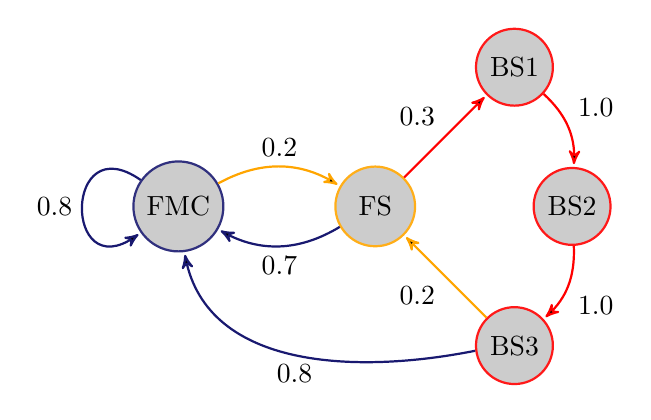
\begin{tikzpicture}[node distance=2.5cm]		
		\node[goodnode] (FMC) {FMC};
		\node[okaynode] (FS) [right of=FMC] {\(\ \)FS\(\ \)};
		\node[badnode] (BS1) [above right of=FS] {BS1};
		\node[badnode] (BS2) [right of=FS] {BS2};
		\node[badnode] (BS3) [below right of=FS] {BS3};
		
		\path[togood] (FMC) 	edge [loop left, min distance=12mm, out=145, in=215]  node [left] 	{\(0.8\)} (FMC);
		\path[togood] (FS)  	edge [bend left]  node [below] 	{\(0.7\)} (FMC);
		\path[togood] (BS3) 	edge [bend left, in=120]  node [below] 	{\(0.8\)} (FMC);
		
		\path[tookay] (FMC) 	edge [bend left]  node [above] 	{\(0.2\)} (FS);
		\path[tookay] (BS3) 	edge []  node [below left] 	{\(0.2\)} (FS);
		
		\path[tobad]  (FS) 		edge []  node [above left] 	{\(0.3\)} (BS1);
		\path[tobad]  (BS1) 	edge [bend left=25]  node [above right] 	{\(1.0\)} (BS2);
		\path[tobad]  (BS2) 	edge [bend left=25]  node [below right] 	{\(1.0\)} (BS3);
	\end{tikzpicture}
	\caption{Single Entity DTMC.}
	\label{DTMC}
\end{figure}


\section{Baseline Analysis}

% Baseline analysis - primary analysis questions
% 	How often will the squadron be able to achieve mission success, meeting 8-orbit mission requirements
% 	How long will it take for the squadron become FMC >= 8 aircraft
% 	What is the long-term sortie generation rate?
% 	What is the long-term mission capable aircraft availability rate?

Under the baseline conditions, the squadron can expect to have 8 aircraft fully mission capable
just over 81\% of the time, after resuming normal operating posture.
The changing probability of the squadron being able to fulfill a sortie during the regeneration 
period can be seen in figure \ref{fig:baseline}.
Our model suggests that the expected time for the squadron to be ready to fly its first sortie
is just over 36 hours. This is the middle estimate; for a more risk-conscious time-line
we have assumed that the extraneous factors effecting the differences in set-up time to 
cause time variations to be approximately normal.
With this assumption, we use the first passage time and variance to examine the next two 
ATO cycles after the third, and determine that there is a probability of
81\% that the squadron will fly its first sortie in or before the fourth
and a 97\% by the end of the fifth.

Using the long term probabilities of each of the states, we estimate that the 
squadron will average 8.88 FMC aircraft for any given ATO, and ultimately
that once expected ops tempo has been reached, the squadron should average
8 sorties in a five day period.

\begin{figure}
	\centering
	\includegraphics[width=0.7\linewidth]{Images/baseline}
	\caption{}
	\label{fig:baseline}
\end{figure}


\section{Exploratory Analysis}

% Sensitivity (excursion) analyses - the what-if questions, 
% 	explore possible solutions by modifying parameter values

In this section we examine the expected effects of changes to different
parts of the system.
Impacts of both positive and negative effects on each part of the squadron's 
maintenance cycles to inform which offer the greatest improvement, 
and which are the greatest liability if disrupted.
Because we do not have access to the costs of improvements, 
it is left to leadership to determine which courses of action will provide
the greatest return on investment.
The requested statistics are consolidated in table \ref{statsTable}.

\subsection{Backshop}
Here we examine the effect of \(\pm\) 10\% to the probability of aircraft 
being approved to return to flight duty as opposed to needed a follow up in the
front shop. Figure \ref{backshopimpairment} shows the effect of a 30\% return 
to the frontshop (up from 20\%). Figure \ref{fig:frontshopimprovement} shows the
effect of only 10\% returning to the frontshop.
This analysis shows that these changes have fairly small effects overall.

\begin{figure}
	\centering
	\includegraphics[width=0.7\linewidth]{Images/BackshopImpairment}
	\caption{}
	\label{fig:backshopimpairment}
\end{figure}
\begin{figure}
	\centering
	\includegraphics[width=0.7\linewidth]{Images/BackshopImprovement}
	\caption{}
	\label{fig:backshopimprovement}
\end{figure}

\subsection{Frontshop}
Figures \ref{fig:frontshopimpairment} and \ref{fig:frontshopimprovement}
examine the effects of a 10\% decrease and increase in positive 
frontshop outcomes, respectively. Here, it can be seen that this effect is more
pronounced than that of the backshop.

\begin{figure}
	\centering
	\includegraphics[width=0.7\linewidth]{Images/FrontShopImpairment}
	\caption{}
	\label{fig:frontshopimpairment}
\end{figure}
\begin{figure}
	\centering
	\includegraphics[width=0.7\linewidth]{Images/FrontShopImprovement}
	\caption{}
	\label{fig:frontshopimprovement}
\end{figure}

\subsection{Post-flight Impairment}

Figures \ref{fig:postflightimpairment} and \ref{fig:postflightimprovement}
show the effects of 10\% decrease and increase in positive outcomes
from the post-flight inspection respectively.
Here, we may see that there is a very pronounced effect.
It seems intuitive that preventing necessary maintenance and 
inspections has a profound effect by avoiding all of the possible
outcomes that may follow.

\begin{figure}
	\centering
	\includegraphics[width=0.7\linewidth]{Images/PostflightImpairment}
	\caption{}
	\label{fig:postflightimpairment}
\end{figure}
\begin{figure}
	\centering
	\includegraphics[width=0.7\linewidth]{Images/PostflightImprovement}
	\caption{}
	\label{fig:postflightimprovement}
\end{figure}

\subsection{Number of Aircraft}
Figures \ref{fig:lostaircraft} and \ref{fig:additionalaircraft}
show the effects of losing an aircraft or if the squadron gained another.
From these analyses we can see that the effective change in number of
aircraft in the squadron (perhaps surprisingly) halve or nearly double the number
of missed sorties.

\begin{figure}
	\centering
	\includegraphics[width=0.7\linewidth]{Images/LostAircraft}
	\caption{}
	\label{fig:lostaircraft}
\end{figure}
\begin{figure}
	\centering
	\includegraphics[width=0.7\linewidth]{Images/AdditionalAircraft}
	\caption{}
	\label{fig:additionalaircraft}
\end{figure}

\subsection{Aircraft Requirement}
Finally, figures \ref{fig:increasedsortierequirement} and \ref{fig:decreasedsortierequirement}
show the effects of changing the requirement to execute a sortie by one,
increasing and decreasing respectively.
Here we see a similar, but more pronounced effect to changing the number
of aircraft in the squadron as a whole.

\begin{figure}
	\centering
	\includegraphics[width=0.7\linewidth]{Images/IncreasedSortieRequirement}
	\caption{}
	\label{fig:increasedsortierequirement}
\end{figure}
\begin{figure}
	\centering
	\includegraphics[width=0.7\linewidth]{Images/DecreasedSortieRequirement}
	\caption{}
	\label{fig:decreasedsortierequirement}
\end{figure}


\section{Conclusions and Recommendations}
From the sensitivity analysis performed on the different parts of the
squadron's operations, we have determined the relative effects on the 
total long-term sortie generation.

\subsubsection{Resiliency of Operations}
The three largest threats to accomplishing the sorties as described
are losing an aircraft, increasing the number required to sortie,
and increased failure of post-flight inspections.

While mission requirements are likely to control the number of aircraft required 
for each ATO, the other two may be more within the control of the squadron.
Avoidance of loss of the aircraft is obvious and already the standard.
Therefore, the most likely place to find improvements to the resilience within 
the squadron will be related to the rates in which aircraft pass or fail the post-flight inspection.
Investigation into possible changes in operating procedures or best practices at this 
point will likely have the most profound effect on improving the squadron's effectiveness,
and may avert the need for costly (in time and money) repairs.

\subsubsection{Improving Sortie Generation}
Improving the post-flight inspections outcomes will improve resilience for the squadron,
and will also have the effect of increasing the number of sorties that can be completed.

The requirement of aircraft to perform sorties should also be examined.
If some ATOs can be accomplished with fewer than eight aircraft, leveraging this
would result in substantial increases in the squadron's ability to accomplish sorties,
likely even higher than if it could acquire additional aircraft,
and would be much more cost effective.

That said, if additional aircraft could be requisitioned it is the third most beneficial action.
Understanding that this is also likely the most expensive course, the third recommendation is to 
evaluate the processes of the front shop with the intention of improving outcomes there.
If there are tools that the maintainers could use to increase the probability of success,
these would likely be significant value added.
However, the most important thing that could be done here is to collect data on which types of
failure send aircraft to the backshop most often.
If the replacement parts for the most common failures can be pre-emptively provisioned
the squadron should have significant increases in sortie generation.

\newcommand\rowHeight{7pt}
\begin{landscape}
\begin{table}[H]
	\begin{tabular}{c|c|c|c|c}
		           Scenario             & Avg. First Sortie (ATO) & Variance & Long Term \% Success & Long-Term Acft FMC per ATO \\ \midrule
		           Baseline             &          3.109          &  0.948   &       81.126\%       &           8.883            \\
		[\rowHeight]
		 Backshop -10\%  &          3.350          &  1.347   &       79.417\%       &           8.794            \\
		[\rowHeight]
		 Backshop +10\%  &          2.300          &  0.650   &       82.699\%       &           8.969            \\
		[\rowHeight]
		Frontshop -10\%  &          3.424          &  1.739   &       71.429\%       &           8.402            \\
		[\rowHeight]
		Frontshop +10\%  &          2.871          &  0.544   &       89.376\%       &           9.383            \\
		[\rowHeight]
		Postlfight -10\% &          3.640          &  2.670   &       54.833\%       &           7.662            \\
		[\rowHeight]
		Postlfight +10\% &          2.785          &  0.439   &       98.053\%       &           10.388           \\
		 [\rowHeight]
		  11 Aircraft   &          3.687          &  2.052   &       64.643\%       &           8.004            \\
		 [\rowHeight]
		  13 Aircraft   &          2.790          &  0.602   &       91.468\%       &           9.816            \\
		 [\rowHeight]
		  9 per Sortie  &          3.990          &  3.233   &       56.384\%       &           9.198            \\
		 [\rowHeight]
		  7 per Sortie  &          2.584          &  0.449   &       95.033\%       &           8.679
	\end{tabular}
	\caption{Consolidated Statistics}
	\label{statsTable}
\end{table}
\end{landscape}

\end{document}